
\documentclass{IOS-Book-Article}

\usepackage{mathptmx}
\usepackage{soul}\setuldepth{article}
\usepackage{graphicx}
\graphicspath{ {./figures/} }


\usepackage {multirow}
%\usepackage [english]{babel}
%\usepackage{setspace}
\usepackage{booktabs}
\usepackage{array}
\usepackage{tabularx}
%\usepackage{calc}
\usepackage{makecell}
\usepackage{array}
\newcolumntype{?}{!{\vrule width 1pt}}


%\usepackage{times}
%\normalfont
%\usepackage[T1]{fontenc}
%\usepackage[mtplusscr,mtbold]{mathtime}
%
\def\hb{\hbox to 11.5 cm{}}

\begin{document}

\pagestyle{headings}
\def\thepage{}
\begin{frontmatter}              % The preamble begins here.


%\pretitle{Pretitle}
\title{First Steps towards a Risk of Bias Corpus of Randomized Controlled Trials}

\markboth{}{April 2022\hb}
%\subtitle{Subtitle}
\author[]{\fnms{Anonymous submission} } 
%\author[A,B]{\fnms{Anjani} \snm{Dhrangadhariya}\orcid{0000-0003-1691-1338}%
%\thanks{Corresponding Author: Anjani Dhrangadhariya, Informatics Institute, HES-SO Valais-Wallis, Technopole 3,
%3960 Sierre, Switzerland; E-mail:
%anjani.dhrangadhariya@hevs.ch.}},
%\author[C,D]{\fnms{Roger} \snm{Hilfiker}}
%,
%\author[C,D]{\fnms{Martin} \snm{Sattelmayer}}
%,
%\author[C,D]{\fnms{Katia} \snm{Giacomino}}
%,
%\author[C,D]{\fnms{Rahel} \snm{Caliesch}}
%,
%\author[C,D]{\fnms{Simone} \snm{Elsig}}
%,
%\author[E,F]{\fnms{Nona} \snm{Naderi}}
%and
%\author[A,B]{\fnms{Henning} \snm{M\"uller}}

%\runningauthor{A. Dhrangadhariya et al.}
%\address[A]{Informatics Institute, HES-SO Valais-Wallis, Sierre, Switzerland}
%\address[B]{University of Geneva (UNIGE), Geneva, Switzerland}
%\address[C]{School of Health Sciences, HES-SO Valais-Wallis, Leukerbad, Switzerland.}
%\address[D]{Department of Physiotherapy, HES-SO Valais-Wallis, Leukerbad, Switzerland.}
%\address[E]{Geneva School of Business Administration, HES-SO Geneva, Switzerland.}
%\address[F]{SIB Swiss Institute of Bioinformatics (SIB), Geneva, Switzerland}

\begin{abstract}
Risk of bias (RoB) assessment of randomized clinical trials (RCTs) is vital to conducting systematic reviews. 
Manual RoB assessment for hundreds of RCTs is a cognitively demanding, lengthy process and is prone to subjective judgment. 
Supervised machine learning (ML) can help to accelerate this process but requires a hand-labelled corpus.
There are currently no RoB annotation guidelines for randomized clinical trials or any annotated corpora.
In this pilot project, we test the practicality of directly using the revised Cochrane RoB 2.0 guidelines for developing an RoB annotated corpus using a novel multi-level annotation scheme.
We report inter-annotator agreement among four annotators who used Cochrane RoB 2.0 guidelines.
The agreement ranges between 0\% for some bias classes and 76\% for others.
Finally, we discuss the shortcomings of this direct translation of annotation guidelines and scheme and suggest approaches to improve them to obtain an RoB annotated corpus suitable for ML.
\end{abstract}

\begin{keyword}
risk of bias\sep annotation\sep
systematic reviews\sep corpus\sep automation
\end{keyword}
\end{frontmatter}
\markboth{April 2022\hb}{April 2022\hb}
%\thispagestyle{empty}
%\pagestyle{empty}
%
%
%
\section{Introduction}
\label{sec:intro}
%
Systematic reviews (SRs) synthesized from randomized controlled trials (RCTs) are the highest quality of evidence in the evidence hierarchy.
In theory, an RCT accurately measures the treatment effect on patient outcomes but can be biased in practice due to flawed study design, execution, analysis or outcome reporting.~\cite{hariton2018randomised}
Biases in RCTs cannot be measured but risk bias can be assessed.
So the reviewers must rigorously look for possible biases before incorporating them into SRs.
Published RCTs are exponentially increasing~\footnote{\url{https://pubmed.ncbi.nlm.nih.gov/?term=randomized\%20controlled\%20trial&filter=pubt.randomizedcontrolledtrial}} over time, making manual assessment a protracted process.
Machine learning (ML) can help accelerate this process by directly pointing the reviewers to the parts of the text relevant to identifying RoB, leading to quickly judging the trial quality.
Both Marshall \textit{et al.} and Millard \textit{et al.} attempted automated RoB assessment, albeit using proprietary, pay-walled data.~\cite{marshall2015automating,millard2016machine}
Recently, Wang \textit{et al.} released a hand-labelled RoB corpus but for preclinical animal studies and not RCTs.~\cite{wang2022risk}
RoB assessment of RCTs is a knowledge-heavy task where even highly trained experts are prone to subjective judgments.
Developing such a corpus entails creating a clear-cut annotation scheme and guidelines, and as neither exists, we focus on two primary concerns:
1) To test whether the widely used revised Cochrane's RoB 2.0 tool for RCTs (RoB 2.0) could be used as RoB annotation guidelines to develop a corpus that could be used for training supervised ML models.
2) To develop and test an RoB annotation scheme that closely mimics the RoB 2.0.~\cite{lansbury2020co,sterne2019rob}
%
%
%
\section{Methods}
\label{sec:methods}
%
\subsection{Formulating Annotation Scheme}
%
RoB 2.0 tool divides biases into five risk domains which further decompose into several signalling questions (SQ), each corresponding to different parts of the trial design.
Each signalling question prompts the reviewer to look for a piece(s) of factual evidence in the RCT and, depending on the amount of evidence found to respond with one of the five response options: ``Yes'', ``Probably yes'', ``No'', ``Probably no'', or ``No information''.
E.g. to respond to the SQ ``Was the allocation sequence random?'', the reviewers need to identify whether a proper methodology was used for random participant allocation and only if a proper methodology is identified the reviewer responds to this question as ``Yes'' and otherwise ``No''.
We formulated an annotation scheme (see Figure~\ref{fig:ann_scheme}) where each SQ is an entity.
Each entity has five entity labels corresponding to the five response options to that question.
Entities represent the factual evidence from the RCTs, and the entity labels incorporate the reviewer's risk judgment.
%
\begin{figure}[!htbp]
    \centering
    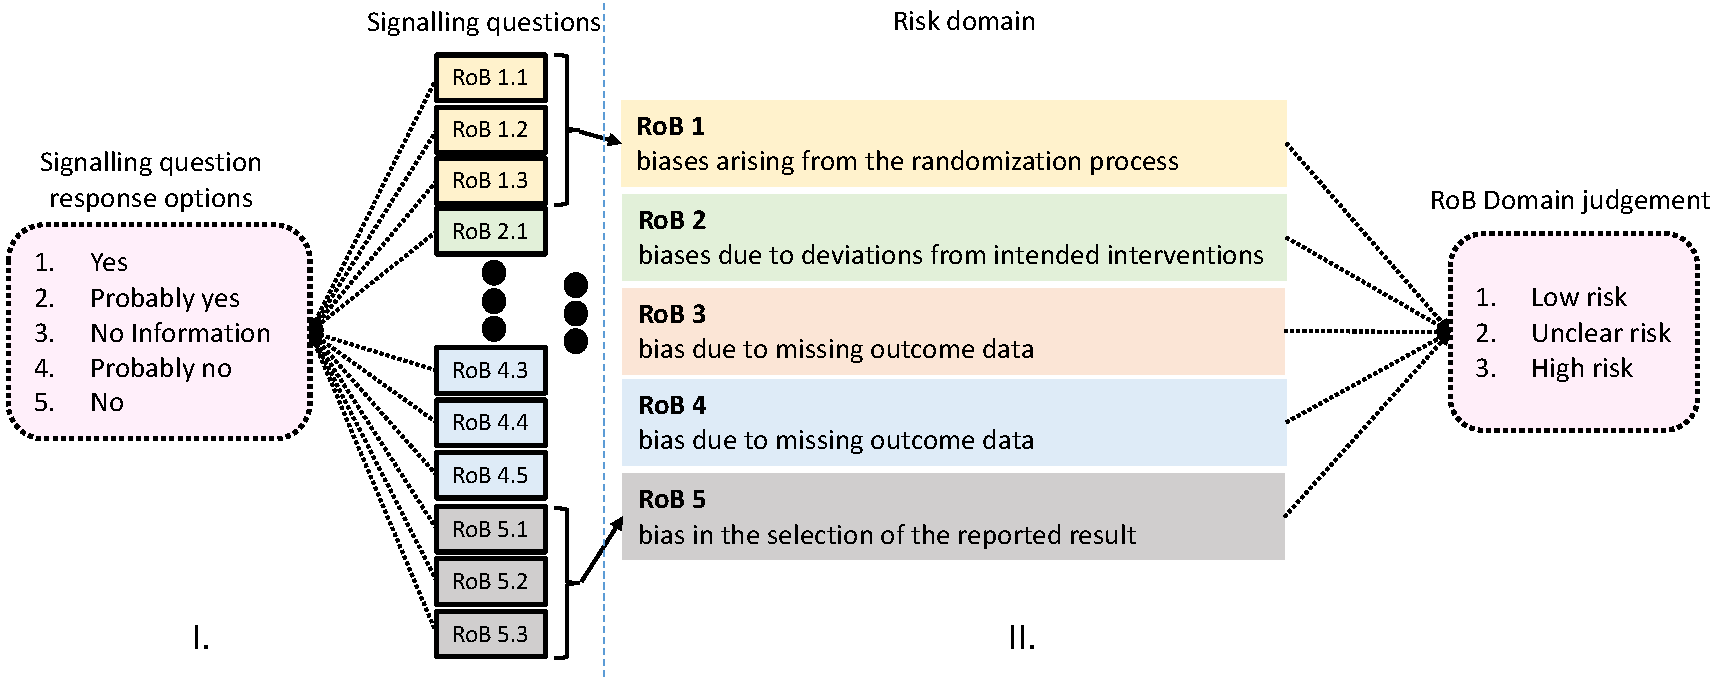
\includegraphics[width=\textwidth]{Figures/annotation_scheme.pdf}
    \caption{Annotation scheme. I. SQ level: each SQ (RoB 1.1, 1.2, ...) is an entity that could take either of five response options (entity labels). SQ response judgements for individual risk domains (RoB 1-5) could be combined to arrive at risk domain judgement. Note: We do not address risk domain judgments in this work.}
    \label{fig:ann_scheme}
\end{figure}
%
%
%
\subsection{Preliminary Annotation guidelines}
\label{subsec:annot_guide}
%
Full-text RCTs were annotated using the RoB assessment instructions from the RoB 2.0.~\footnote{\url{https://drive.google.com/file/d/19R9savfPdCHC8XLz2iiMvL_71lPJERWK/view}}
The author with NLP (Natural Language Processing) expertise developed the generic annotation guidelines with four physiotherapists experienced in bias assessment to ensure consistency.
Complete sentence(s) or phrase(s) were annotated depending upon the text parts relevant to answering a SQ.
All the text information pertinent to answering a question was marked, even if the information was found in different parts of the full text.
Table or figure captions relevant to answering were marked.
If the information was not found in the captions, it was marked within the table contents.
If a reference to the table or figure led to answering the question, it was annotated.
If all three were relevant then all were annotated.
%
\subsection{Pilot annotation}
\label{subsec:annotation}
%
The four physiotherapists, who consented to annotating, did the pilot annotation on a corpus of ten RCTs sampled in the following manner.
An Entrez~\footnote{The Entrez Global Query Cross-Database Search System is a federated search engine or web portal that allows users to search PubMed database} search using the search query ``{\fontfamily{qcr}\selectfont (randomized[title] or randomized[title]) and (rehabilitation or (physical therapy))}'' was performed ten times to retrieve studies from one-year time-spans each between 2000 - 2019.
Each query was restricted to retrieve 1000 documents, of which ten were randomly chosen for each time span.
Of the ten sampled studies, we took the first possible study with a freely available PDF (Portable Document Format).
Two of the annotators are professors and associate professors, and the other two are doctoral researchers with experience conducting RoB ratings in several SRs.
Tagtog\footnote{\url{https://www.tagtog.com/}}, a commercial tool, was used for annotating the PDFs.
The task was to annotate text relevant to answering each signalling question entity and choose a judgment response option entity label.
%and finally select the risk domain judgment for the five risk domains.
We report token-level pairwise F1 measure as an inter-annotator agreement (IAA) for the entity $IAA_{sq}$ and entity label $IAA_{response}$ annotations.~\cite{deleger2012building}
$IAA_{sq}$ and $IAA_{response}$ measure reliability of the RoB 2.0 guidelines for selecting the same parts of the text to answer SQs.
%Cohen's Kappa was chosen for the document-level $IAA_{rd}$ agreements.~\cite{mchugh2012interrater}
%
%
%
\section{Results}
\label{sec:results}
%
The pilot annotation resulted in 902 labels corresponding to the SQs and their response options.
The Table \ref{tab:iaa_sq_res} reports pairwise $IAA_{sq}$ and $IAA_{response}$ averaged over all the annotator pairs at the SQ response option level.
Individual pairwise $IAA_{sq}$ range between 0\% (poor) and 75\% (substantial), with most values falling under the poor category and very few under the substantial agreement.
SQs RoB 1.1, 1.2, 1.3, 2.6, and 3.1 fared well in terms of the average pairwise agreement between all pairs, but none of these categories had a substantial agreement.
Questions 2.1, 2.3, 2.4, 2.5, 2.7, 3.4, 4.4, 4.5, and entire domain 5 fared extremely poorly or with no agreement or no annotation.
The $IAA_{response}$ scores are considerably lower (to zero) than $IAA_{sq}$, hinting that annotators choose the same text to answer a SQ but assign different response options to the selected text. 
The $IAA_{response}$ scores remain variable across the risk domains with 52.63\% of the total scores being zero and no annotation for about 22\% of the total scores.
%
\begin{table}[!ht]
    \centering
    \begin{tabular}{c?c|c|c|c|c|c|c?c|c|c|c|c}
    %\hline
        SQ & P1 & P2 & P3 & P4 & P5 & P6 & Avg. & Y & PY & NI & PN & N \\
    \Xhline{1.0pt}
        1.1 & 23.1 & 24.5 & 52.2 & 57.0 & 48.0 & 21.5 & 37.7 & 21.8 & 7.1 & 0.0 & - & - \\ 
        1.2 & \textbf{66.1} & 50.3 & 72.8 & 50.7 & 46.0 & 50.5 & 56.1 & 4.9 & 11.5 & 10.2 & 0.0 & - \\ 
        1.3 & \textbf{69.5} & 20.5 & 16.1 & 31.6 & 59.9 & 53.5 & 41.8 & - & - & 41.8 & 11.4 & 9.9 \\ \hline
        2.1 & 1.0 & 1.4 & 0.0 & 9.1 & 19.1 & 0.0 & 5.1 & 8.2 & 0.0 & - & 3.0 & 0.0 \\ 
        2.2 & 18.3 & 7.3 & 11.1 & 0.0 & 23.0 & 7.4 & 11.2 & 3.6 & 0.0 & 0.0 & 0.0 & 0.0 \\ 
        2.3 & 20.6 & 5.5 & 13.4 & 0.0 & 0.0 & 0.0 & 6.6 & - & 0.0 & - & 1.0 & 0.0 \\ 
        2.4 & 0 & - & - & 0 & 0 & - & 0 & - & 0 & - & 0 & - \\ 
        2.5 & 0 & 0 & 0 & 0 & 0 & - & 0 & 0 & 0 & - & 0 & - \\ 
        2.6 & \textbf{75.3} & \textbf{68.9} & 19.3 & \textbf{63.9} & 12.9 & 19.6 & 43.3 & 39.4 & 0.0 & 0.0 & 0.0 & 3.6 \\ 
        2.7 & 0.0 & 6.6 & 0.0 & 0.0 & 0.0 & 0.0 & 1.1 & 0.0 & 0.0 & - & 0.0 & 0.0 \\ \hline
        3.1 & 45.8 & 23.6 & 32.2 & 43.4 & 22.9 & 14.8 & 30.4 & 47.6 & 0.6 & - & 1.3 & 3.3 \\ 
        3.2 & 1.4 & 0.0 & 0.0 & 3.3 & 7.4 & 0.9 & 2.2 & 0.0 & 0.0 & - & 0.0 & 0.0 \\ 
        3.3 & 0.0 & 0.0 & 0.0 & 16.4 & 0.0 & 0.0 & 2.8 & - & 0.0 & 31.4 & 0.0 & 0.0 \\ 
        3.4 & - & 0 & - & 0 & 0 & 0 & 0 & 0 & 0 & 0 & 0 & 0 \\ \hline
        4.1 & 4.0 & 6.6 & 14.2 & 25.6 & 22.3 & 6.3 & 13.2 & - & - & - & 0.8 & 12.0 \\ 
        4.2 & 1.8 & 0.0 & 0.4 & 0.0 & 40.1 & 0.0 & 7.1 & - & - & - & 0.3 & 0.0 \\
        4.3 & 7.6 & 13.9 & 5.0 & 10.5 & 39.5 & 8.4 & 14.2 & 0.0 & 0.0 & 0.0 & 13.1 & 20.5 \\ 
        4.4 & 0 & 0 & 0 & 0 & 0 & 0 & 0 & 0 & 0 & - & 0 & 0 \\ 
        4.5 & 0 & 0 & 0 & 0 & 0 & 0 & 0 & 0 & 0 & - & 0 & - \\ \hline
        5.1 & 0.0 & 0.0 & 0.0 & 0.0 & 0.0 & 4.2 & 0.7 & 0.0 & 0.0 & 0.0 & 0.0 & 0.0 \\ 
        5.2 & 23.9 & 0.0 & 0.0 & 0.0 & 0.0 & 2.4 & 4.4 & - & 0.0 & 0.0 & 0.0 & 0.0 \\ 
        5.3 & 0.2 & 0.0 & 0.0 & 0.4 & 8.1 & 42.0 & 8.4 & - & 0.0 & 0.6 & 0.0 & 0.0 \\
    \Xhline{1.0pt}
    \end{tabular}
    \vspace{1em}
    \caption{\label{tab:iaa_sq_res} Left: Table lists down $IAA_{sq}$ between the six annotator pairs (P1-P6) for the RoB SQs. Substantial ($\geq$ 61) agreements are in bold. Right: Table lists down $IAA_{sq}$ averaged over the six annotator pairs for the SQs at the ``response'' option or entity label level. Note: Y = Yes, PY = Probably Yes, NI = No Information, N = No and PN = Probably No, Avg. = Average. “-” shows that one of the annotators did not annotate any text for a particular SQ.}
\end{table}
%
%
%
\section{Discussion}
\label{sec:disc}
%
Annotation analysis identified four types of disagreements. 
A \textbf{polarity disagreement} arises when two annotators choose the same chunk of text to answer a SQ but choose polar opposite entity labels (``Yes'' or ``Probably yes'' vs ``No'' or ``Probably no'' vs ``No information'').
In one of the documents, all four annotators chose the same text evidence (``71 allocated routine services, 67 allocated intervention service, ...'') to answer the SQ 3.1.
However, three of the four annotators responded to this question with ``Yes'', but one chose ``Probably no''.
This SQ asks whether the outcomes data were available for all, or nearly all, participants randomized but does not clarify the exact cut-off for how many participant dropouts increase the risk?
Therefore, the annotators make subjective response judgments depending upon what exact percentage of participant dropout is considered valid in their experience.
A \textbf{degree disagreement} causes low $IAA_{response}$ and arises because some annotators are lenient in judging risk while others are sceptical.
The lenient ones select definitive ``Yes'' or ``No'' for responding to a SQ, while the sceptical ones choose ``Probably yes'' or ``Probably no''.
A practical and rationally justified solution is to merge the response options ``Probably yes'' with ``Yes'' and ``Probably no'' with ``No'' to reduce the complexity of the task and increase IAA without altering the final risk judgment for this risk domain.~\cite{sterne2019rob}
A low IAA is also caused by our annotation guidelines not limiting the annotators to selecting either the phrase vs a sentence(s) vs a paragraph for answering the question leading to a \textbf{text span disagreement}.
RoB 2.0 tool led to some annotators using and annotating very condensed information to come to a response.
In contrast, others used an entire paragraph to reach the same response for a SQ leading to a low token-level IAA.
This problem requires mending the annotation guidelines to precisely instruct authors to select the complete information they used to decide or the minimum necessary information to decide on a SQ.
Another method is automatically extending the more condensed annotations to the broadest ones.
In our guideline improvement, we are restricting the annotation to marking the full sentence(s) where the relevant information is found.
Sometimes annotators came to a response judgment for a SQ but used different parts of the RCT text leading to \textbf{disparate document section disagreement}.
Such disagreements emanate because RoB 2.0 guidelines do not instruct the annotators about what part of the RCT to annotate and what part to not annotate for a particular SQ.
We noticed many SQs remained unanswered because the annotators did not understand what part of the text to annotate, even after following the RoB 2.0 guidelines.
%
%
%
\section{Conclusion}
\label{sec:conclusion}
%
In conclusion, RoB 2.0 cannot be directly used as corpus annotation guidelines.
It is imperative to develop clear-cut guidelines to instruct the annotators in SQ and response judgment decisions.
The multi-level annotation schema also needs improvement.
We are using the insights from this pilot annotation to develop detailed, crisp guidelines to obtain consistent annotations. 
The annotated dataset is available on Zenodo.
%
%
%
%%%%% References %%%%%
\bibliographystyle{spiebib} 
%
%
\bibliography{bibliography}
%
\end{document}
